\subsection{Explicit preference information at matched counts}
The exploratory follow-up recorded 2,400 completed receipt requests, with no delivery failures. Both models returned their requested snapshots and correctly reported the largest supplied weight on every calibration and field request. This is accuracy on 12 repeated, explicitly specified prompts, not evidence of general preference understanding. The two models therefore induce identical empirical receipt channels and identical receipt intervals on the shared task subset.

Each model's receipt channel resolves three of nine primary follow-up conditions, compared with zero of nine using the matched original actions. All three resolved conditions are the positive cohort, one per domain; none contradicts the known synthetic target. The negative and near cohorts remain unresolved. Mean interval width decreases from 0.0872 for action logs to 0.0436 for receipts, a 50.0\% reduction. These figures summarize the selected conditions and do not constitute a significance test or a post-selection coverage guarantee.

\begin{table}[t]
\centering\small
\begin{tabular}{@{}lrr@{}}
\toprule Paired measure, per model & Actions & Receipts \\\midrule
Calibration per class/domain & 40 & 40 \\
Field per cohort/domain & 80 & 80 \\
Resolved contrasts / conditions & 0 / 9 & 3 / 9 \\
Incorrect resolved contrasts & 0 & 0 \\
Mean interval width & 0.0872 & 0.0436 \\\bottomrule
\end{tabular}
\caption{Exploratory comparison. Both models have the same reported interval summaries. Perfectly reporting the supplied leading attribute directly reveals the constructed intent class. Counts do not equalize monetary cost or elicitation burden.}
\label{tab:receipt}
\end{table}

\begin{figure*}[t]
\centering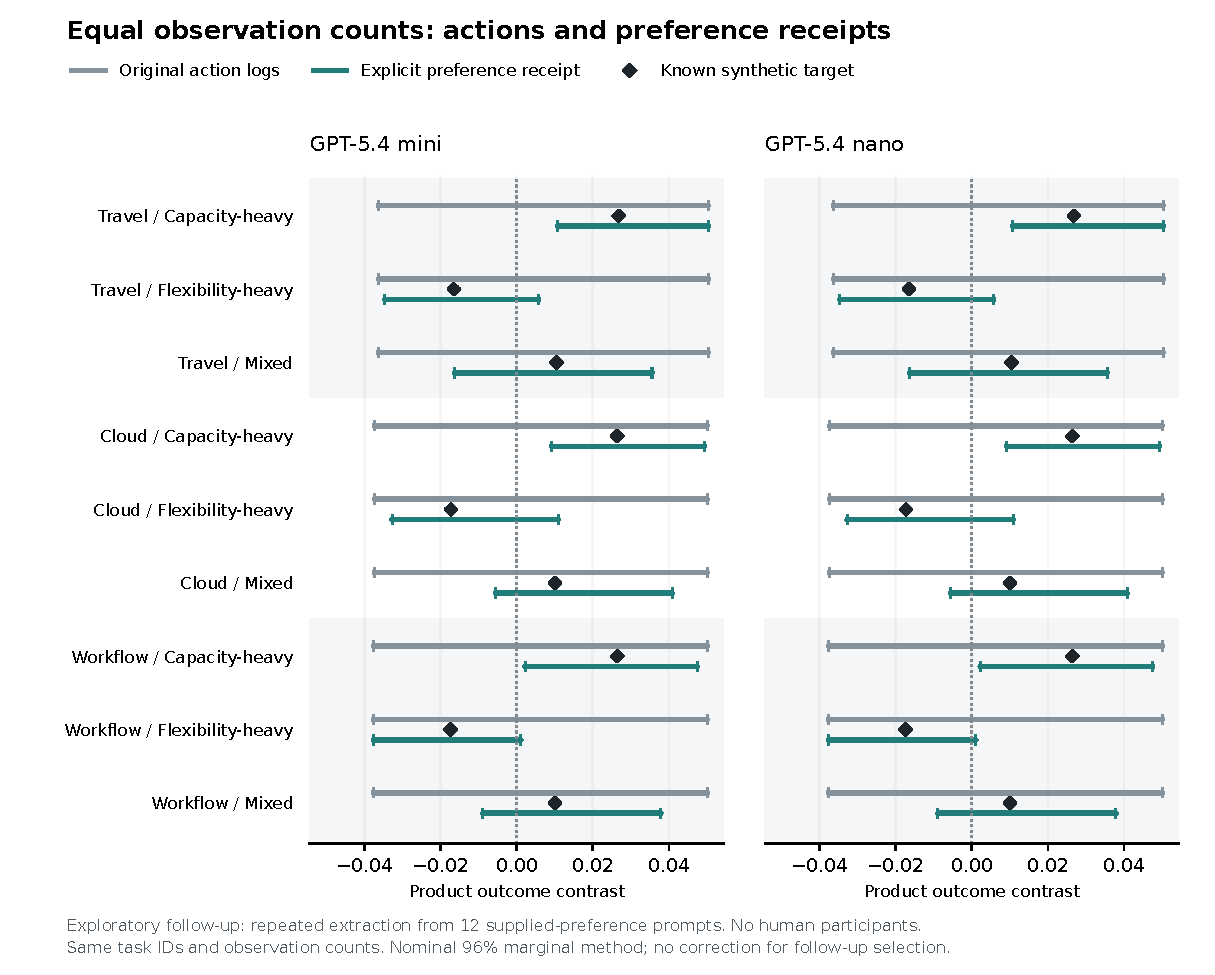
\includegraphics[width=.94\textwidth]{../results/receipt-study-summary/receipt-comparison.pdf}
\caption{Action-only and attribute-only intervals on the same selected task IDs. The receipt collects explicit preference information omitted from the action log; it does not discover an unobserved human preference. The follow-up was chosen after the primary results, so these are exploratory comparisons without selective-inference correction.}
\label{fig:receipt}
\end{figure*}

The result separates two limitations. Even a directly observed class does not resolve every small contrast under this finite-sample procedure. Yet the same number of observations is more useful when it records a relevant class attribute instead of a behavioral proxy. The receipt's remaining uncertainty is sampling and channel-calibration uncertainty within the declared model, rather than a demonstrated loss of the supplied class information. Since a deterministic extractor would provide the same field, this experiment supports explicit measurement design, not the necessity of an LLM receipt generator.

Reported usage implies an additional US\$0.372 for the follow-up. Across the two studies, there are 7,200 attempted API requests, 7,183 valid responses, and 17 retained transport failures. The excluded connectivity test is not part of these counts. All preferences and product outcomes remain synthetic.
